
\documentclass{article}
\usepackage{graphicx}
\usepackage{longtable}
\usepackage{geometry}
\geometry{a4paper, margin=1in}
\graphicspath{{CC:\\Users\\siaha\\PycharmProjects\\Unemployment_House\\Analytics}}

\begin{document}

\title{Sample LaTeX Report with Image and Dataframe}
\author{Your Name}
\date{\today}
\maketitle

\section{Introduction}
This is a simple LaTeX report generated using Python. Below is a plot generated from Python:

\begin{figure}[h!]
\centering
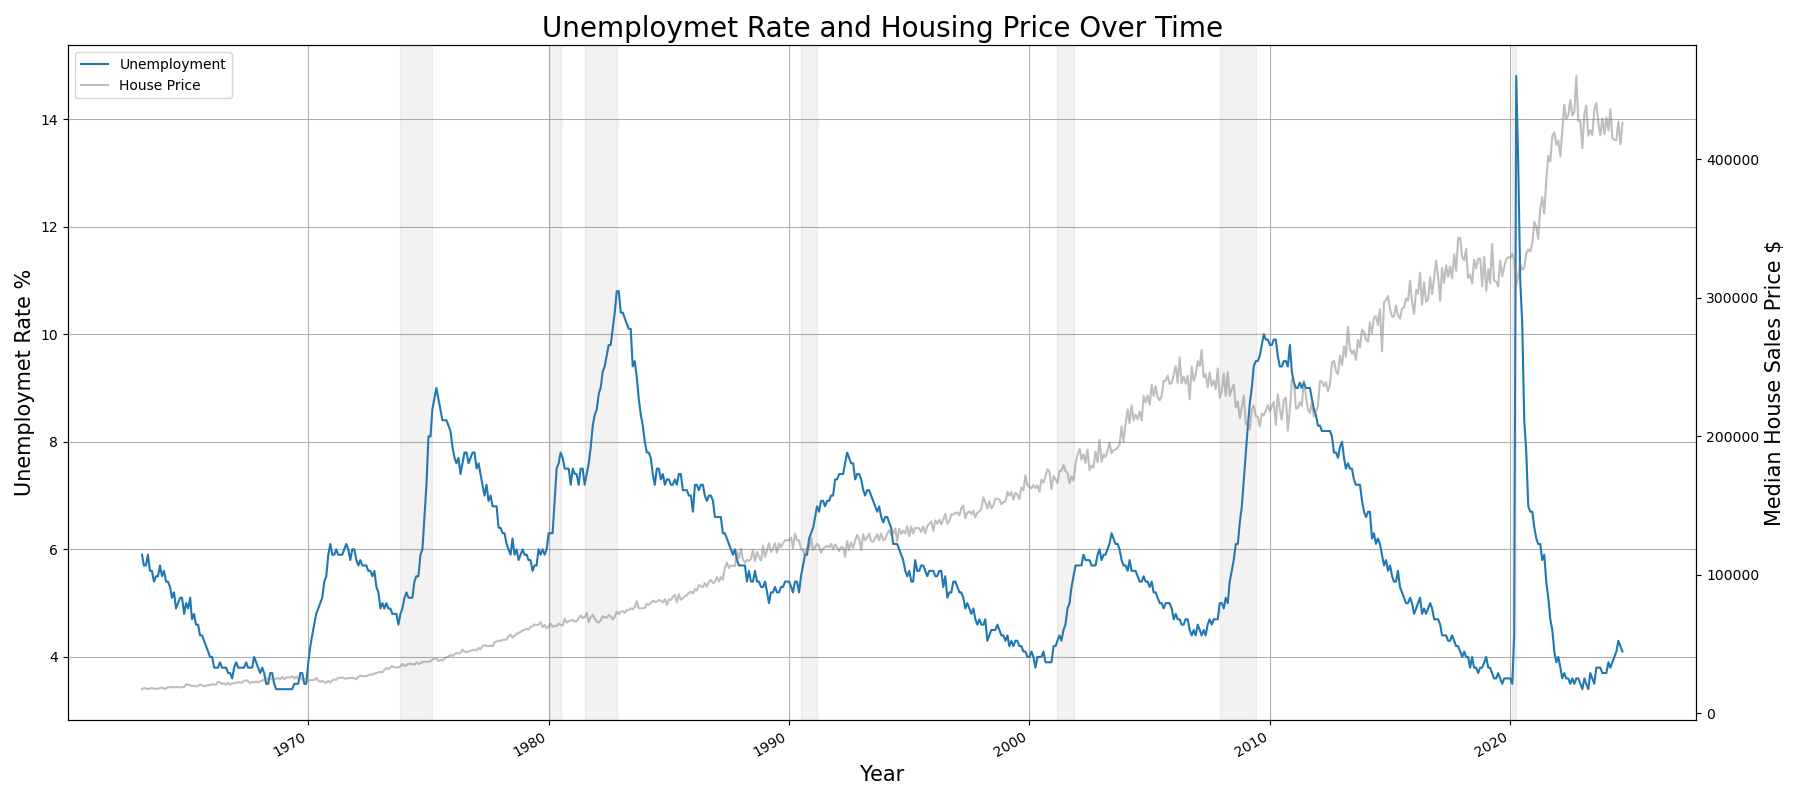
\includegraphics[width=0.8\textwidth]{C:/Users/siaha/PycharmProjects/Unemployment_House/Analytics/timeseries1.png}
\caption{Time Serie Test}
\end{figure}


\section{Dataframe}
The following table represents some sample data:

\begin{longtable}{|c|c|c|}
\hline
\textbf{Index} & \textbf{Value1} & \textbf{Value2} \\
\hline
\endfirsthead
\hline
\textbf{Index} & \textbf{Value1} & \textbf{Value2} \\
\hline
\endhead
Unemployment Rate & 0.01669963578143125 & stationary  \\
Median Housing Price Over Time & 0.9973693419874184 & non-stationary  \\
First diff of housing Price & 1.0845421411142084e-06 & stationary  \\


\end{longtable}

\end{document}
    